
\documentclass[acmsmall, nonacm]{acmart}


\renewcommand\footnotetextcopyrightpermission[1]{} % removes footnote with conference information in first column
\makeatletter
\let\@authorsaddresses\@empty % removes authors' addresses from first page footer
\makeatother


\usepackage{tikz}
\usetikzlibrary{positioning}
\usepackage{xcolor}
\definecolor{mygreen}{RGB}{0,120,0}
\usepackage{wrapfig}
\usepackage{capt-of}

%% (Not sure if this is needed)
%% \BibTeX command to typeset BibTeX logo in the docs
\AtBeginDocument{%
  \providecommand\BibTeX{{%
    \normalfont B\kern-0.5em{\scshape i\kern-0.25em b}\kern-0.8em\TeX}}}


\begin{document}


\title{A Divide-and-Conquer Approach to Discovering Minimal Realizable Grammars}


\author{Will Thomas}
\author{Logan Schmalz}
\author{Sarah Johnson}


\maketitle

\section{Introduction}
%%(Presents the central idea of your project and summarizes the takeaways)

\section{Background}
Our project is based on the work of Semantic-Guided Synthesis (SemGuS) \cite{semgus}. SemGuS aims to be ``a language-agnostic logic-based framework for program synthesis problems over arbitrary semantics''. A SemGuS problem is defined by language syntax given as a Regular Tree Grammar (RTG), language semantics given as Constrained Horn Clauses (CHCs), and problem specification given by logical constraints or input-output examples. The feature that sets SemGuS apart from Syntax-Guided Synthesis (SyGuS) is the ability to define a custom semantics for a language, as SyGuS cannot express problems that contain semantics outside of supported theory. SemGuS accepts recursively defined big-step semantics allowing synthesis over imperative programming languages that contain loops with unbounded behaviour. Kim et al. not only designed the SemGuS framework but also developed an algorithm for solving SemGuS problems. The algorithm encodes SemGuS problems as a proof search over CHCs and is capable of both synthesizing programs and proving unrealizability, the latter of which our project relies on.


\section{Overview}
%%(Gives step by step working of your project on a single example)

 \begin{wrapfigure}{r}{8.1cm}   
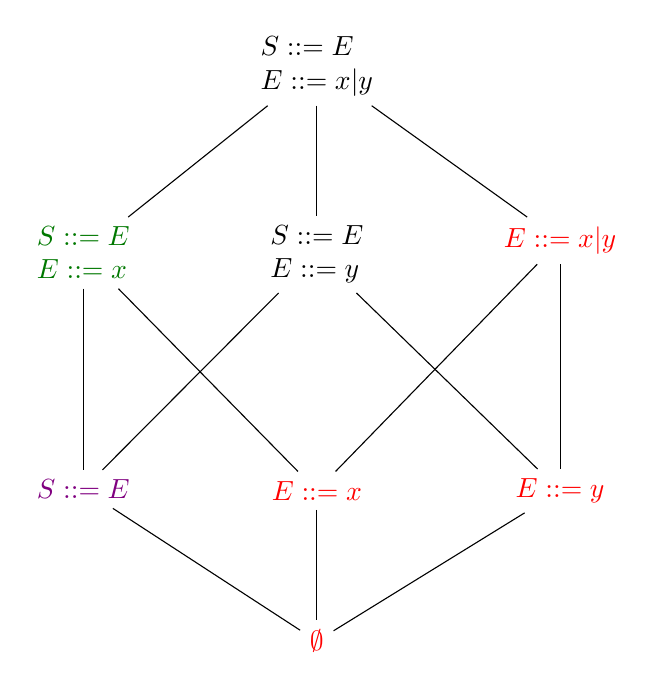
\begin{tikzpicture}[node distance=3cm]
\title{lattice 2}
\node(123)      [align=left]              {$S ::= E$ \\ $E ::= x \text{ }\vert\text{ } y$};
\node(12)       [below left=2cm of 123, align=left] {$\color{mygreen} S ::= E$ \\ $\color{mygreen} E ::= x$};
\node(13)      [below=1.4cm of 123, align=left]  {$S ::= E$ \\ $E ::= y$};
\node(23)      [below right=2cm of 123, align=left]       {$\color{red} E ::= x \text{ }\vert\text{ } y$};
\node(1)      [below of=12]       {$\color{violet} S ::= E$};
\node(2)      [below of=13]       {$\color{red} E ::= x$};
\node(3)      [below=2.6cm of 23]       {$\color{red} E ::= y$};
\node(empty)      [below=1.4cm of 2]       {$\color{red} \emptyset$};

\draw(123)       -- (12);
\draw(123)       -- (13);
\draw(123)       -- (23);
\draw(12)       -- (1);
\draw(12)       -- (2);
\draw(13)      -- (1);
\draw(13)      --  (3);
\draw(23)      --  (2);
\draw(23)      --  (3);
\draw(1)      --  (empty);
\draw(2)      --  (empty);
\draw(3)      --  (empty);
\end{tikzpicture}
\captionof{figure}{Subgrammar Lattice}
\label{fig:lattice}
\end{wrapfigure}

Consider a very simple example problem: synthesize a function that returns the first projection of an ordered pair. Our goal is to find a minimal realizable subgrammar for this problem. The full grammar consists of a start nonterminal symbol $S$ with a single production rule $E$. $E$ is an expression nonterminal symbol with two production rules $x$ and $y$. $x$ returns the first parameter given to the function while $y$ returns the second. In this example, it is obvious to see that $y$ can be removed from the language and the problem is still realizable.

In our work, we design a sound and complete algorithm for finding a minimal realizable subgrammar. Given some grammar, the algorithm generates every subgrammar (including invalid ones) and checks realizability under each one. The total set of subrammars is equal to the power set of the production rules and forms a lattice under the subset relation as shown in Figure \ref{fig:lattice}. The red text denotes invalid grammars due to missing start symbol; the purple text denotes invalid grammars due to missing nonterminal symbol; and the green text denotes the minimal realizable grammar given the behavioural specification.


\section{Technical Details}
%%(If your project has formal theory or algorithms you can present it here in the most general form. While the previous section explained the same thing with an example, this section should be about the general technical ideas under the hood)

\section{Implementation}
%%(The general technical ideas are never enough to get a working implementation :) You probably had to cut corners, optimize certain things to make it practical, etc. which go here)

\section{Evaluation}
%%(The results of running your tool, the benchmarks you ran on and your takeaways from it. Things like we learned this parameter is the key bottleneck, our tool struggles on XYZ, or we did well on ABC)

\section{Conclusion}
%%(Your concluding take on the project and learnings)

\section{Future Work}
%%(Potential future work that you think could be interesting)





\bibliographystyle{ACM-Reference-Format}
\bibliography{projectrefs}


\end{document}

